\chapter{Linear Discriminant Analysis}
\label{chapter:lda}
\section{簡介}
\label{sec:LdaIntroduction}




%Linear Discriminant Analysis(LDA),是一種降維演算法,但與前一節提到的PCA有些許的不同,這個演算法屬於一種「監督式」的學習法,所以在進行演算法的運算時,須考慮資料的類別。

線性區別分析(Linear Discriminant Analysis,LDA),屬於一種「監督式」的降維演算法,所以在進行演算法運算時,須考慮資料的類別。
前一小節提到PCA是希望能在特徵空間中找到一個向量,使得資料的投影點,彼此之間的變異數越大越好。而LDA則是希望能夠找到一個投影向量,使得組內的離散程度越小越好,與組間的離散程度越大越好。




\section{相關參數與實例說明}
為了更簡單理解這個演算法的數學意義,以下舉一個例子說明:


\subsection{相關參數}

\begin{itemize}
	\item
	      \(\mathbf{S_w}\) 為組內離散程度矩陣,不同類別中的資料變異量總合。而 \(\mathbf{{S_w}'}\)是經過投影後的組內離散程度矩陣。
	\item
	      \(\mathbf{S_b}\) 為組間離散程度矩陣,表示兩兩類別之間群心的變異量的總合。\(\mathbf{{S_b}'}\) 為投影後的組間離散程度矩陣。
	\item
	      \(\mathbf{u}\) :所有資料均值。
	\item
	      \(\mathbf{u_i}\) :第i類資料均值。
	\item
	      \(\mathbf{x_i}\) :第i筆資料。
	\item
	      \(n_i\) :屬於i類的資料個數。
	\item
	      \(\mathbf{w}\) :投影軸。
\end{itemize}

\subsection{實例說明}
\begin{itemize}
	\item
	      圖\ref{fig:LdaDemostrate}為一個具有兩個維度的資料分佈圖,分別有黃、藍、灰三類。
	      \begin{figure}[h]
		      \centering
		      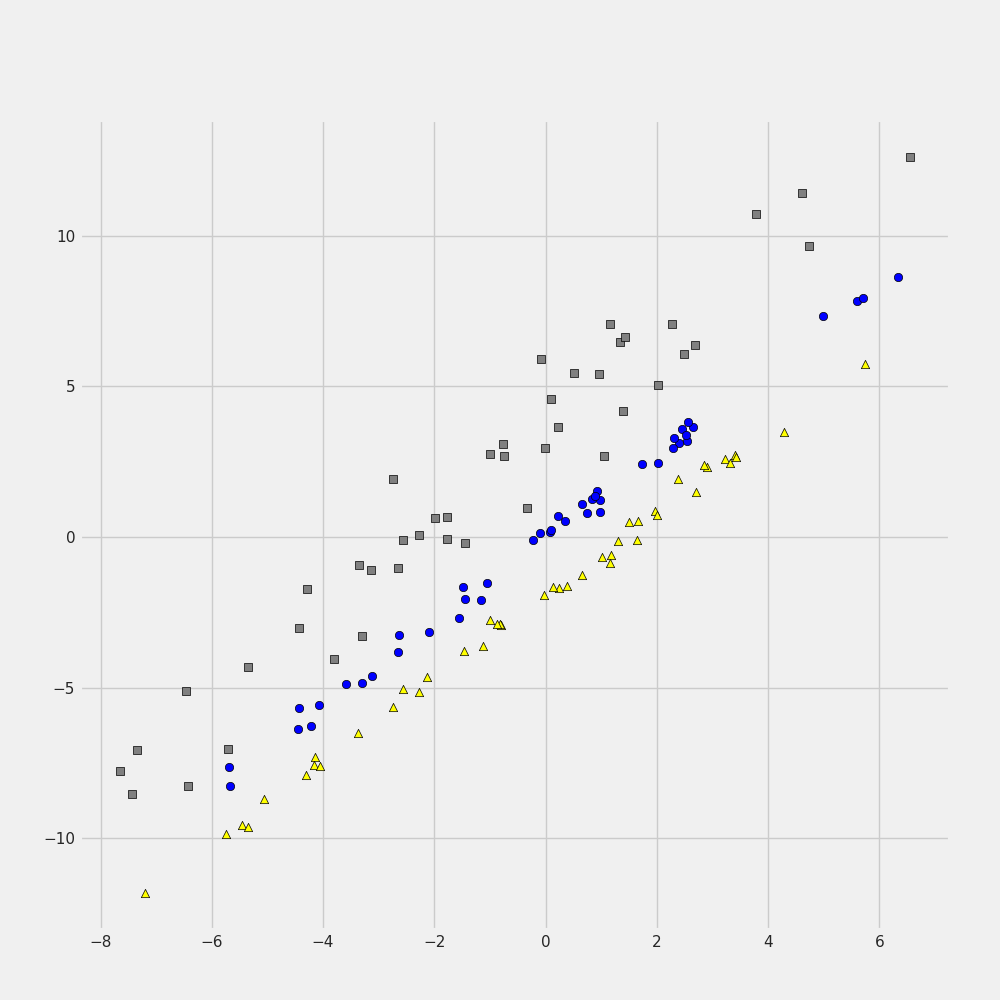
\includegraphics[width=6cm]{pic/lda_dataset.png}
		      \caption{二維資料}
		      \label{fig:LdaDemostrate}
	      \end{figure}


	      %
	\item
	      首先,由式(\ref{eqn:LdaWithin})計算不同類別的變異數總合 \(\mathbf{S_w}\)。並由式(\ref{eqn:LdaWithinTransform})計算經過投影後的組內離散矩陣 \(\mathbf{{S_w}'}\)。

	      %%由式(\ref{eqn:LdaWithinTransform})計算經過「投影後」的組內離散矩陣 \(\mathbf{{S_w}'}\)。其中 \(\mathbf{S_w}\) 為不同類別的變異數總合。

	      \begin{equation}
		      \label{eqn:LdaWithin}
		      \mathbf{S_w}  =\sum_{i=1}^{c} \sum^{}_{x_k\in class}  \mathbf{(x_k - u_i)(x_k-u_i)^T}
	      \end{equation}

	      \begin{equation}
		      \label{eqn:LdaWithinTransform}
		      \begin{aligned}
			      \mathbf{{S_w}'} & =\sum_{i=1}^{c} \sum^{}_{x_k\in class}  \mathbf{(w^Tx_k - w^Tu_i)(w^Tx_k-w^Tu_i)^T}
			      \\& =\mathbf{w^T}(\sum_{i=1}^{c} \sum^{}_{x_k\in class} \mathbf{ (x_k - u_i)(x_k-u_i)^T)w}
			      \\& =\mathbf{w^TS_ww}
		      \end{aligned}
	      \end{equation}


	\item
		接著由式 (\ref{eqn:BetweenClassScatter})計算組間離散程度 \(\mathbf{S_b}\)。並由式 (\ref{eqn:LdaTransformClassScatter})計算「投影後」的組間離散程度 \(\mathbf{{S_b}'}\) 。

	      \begin{equation}
		      \label{eqn:BetweenClassScatter}
		      \mathbf{S_b} =\sum_{i=1}^{c}\sum_{i \neq j } \mathbf{(u_i - u_j)(u_i - u_j)^T}
	      \end{equation}

	      \begin{equation}
		      \label{eqn:LdaTransformClassScatter}
		      \begin{aligned}
			      \\&\mathbf{{S_b}'} =\sum_{i=1}^{c}\sum_{i \neq j } \mathbf{(w^Tu_i - w^Tu_j)(w^Tu_i - w^Tu_j)^T}
			      \\& =\mathbf{w^T}(\sum_{i=1}^{c}\sum_{i \neq j } \mathbf{(u_i - u_j)(u_i - u_j)^T)w}
			      \\& =\mathbf{w^TS_bw}
		      \end{aligned}
	      \end{equation}



	      \begin{figure}[H]
		      \centering
		      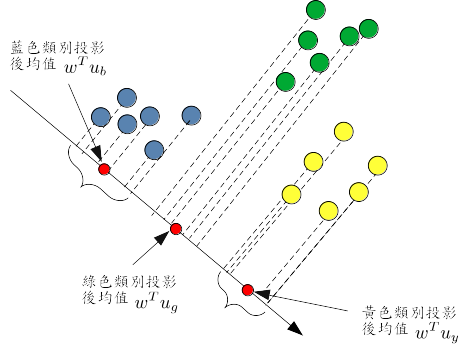
\includegraphics[height=5cm]{./pic/bugfxgEn.png}
		      \caption{部分資料經過投影的結果}
		      \label{fig:LdaTransform}
	      \end{figure}

	\item
	      根據前一小節提到的,希望投影過後「組內離散程度越小越好,組間離散程度越大越好」,最後會希望找到一個 \(w\),使得\(\frac{\mathbf{S_b}}{\mathbf{S_w}}\) 越大越好,如式(\ref{eqn:FindMaximun})。

	      \begin{equation}
		      \label{eqn:FindMaximun}
		      \underset{w}{max}\frac{\mathbf{{S_b}'}}{\mathbf{{S_w}'}} =\underset{w,w^TS_ww = 1}{max}\frac{\mathbf{{S_b}'}}{\mathbf{{S_w}'}}
	      \end{equation}


	      %
	\item
	      最後,圖\ref{fig:LdaDataLdaTransform}為此資料經過LDA轉換的結果,資料變得比較好區分。此外,圖\ref{fig:LdaDataPcaTransform}為經過PCA轉換的結果,雖然比原資料來的好,但是與LDA的結果相比,還是差了一些。
	      \begin{figure}[H]
		      \begin{center}
			      \begin{tabular}{ccccccccccccc}
				      \subfigure[資料經過LDA轉換的結果 ]{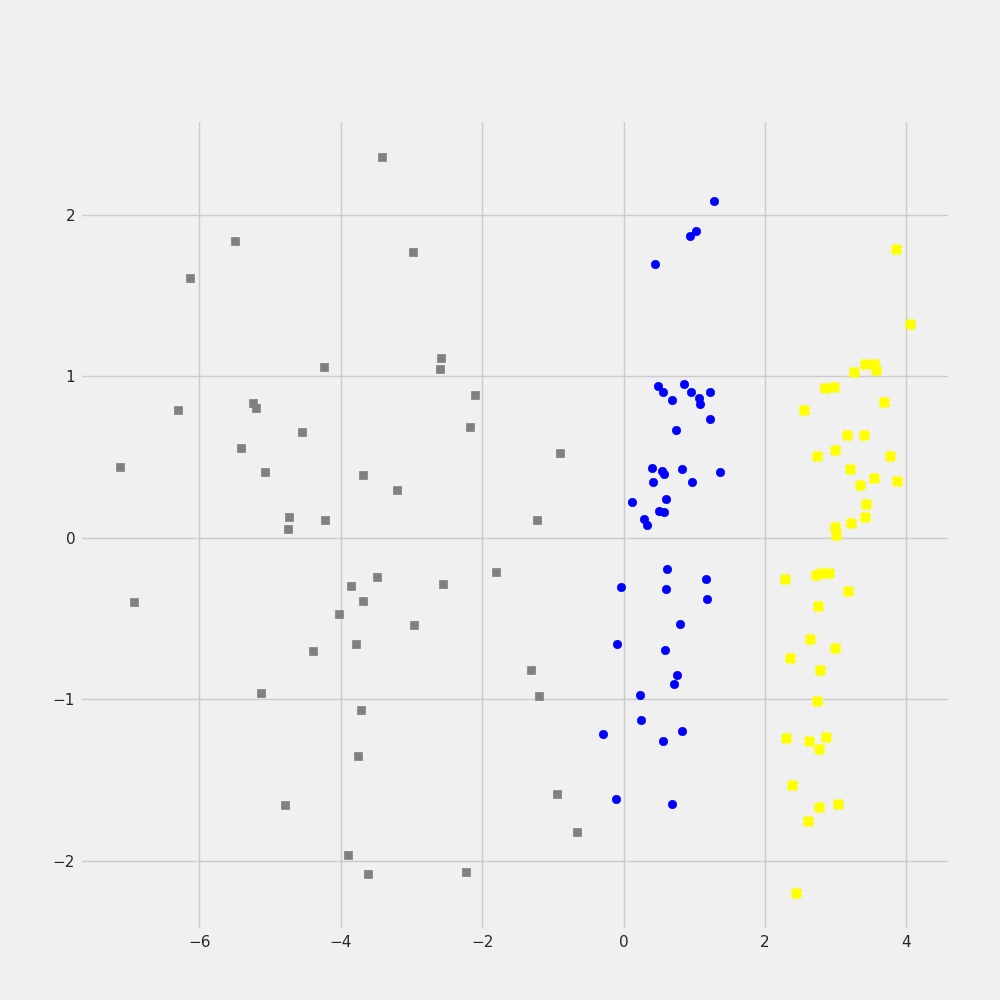
\includegraphics[width=7cm]{pic/lda_dataset_lda_transform.png}\label{fig:LdaDataLdaTransform} } \par &
				      \subfigure[資料經過PCA轉換的結果]{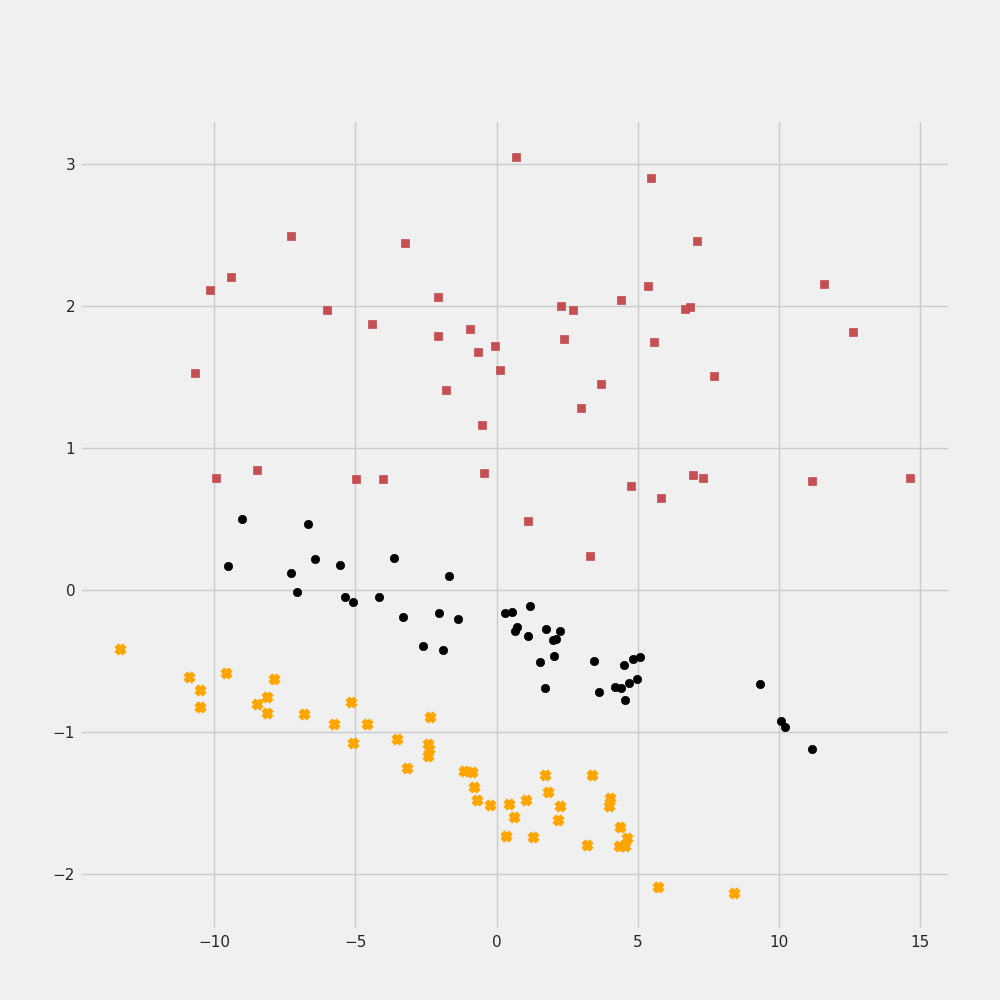
\includegraphics[width=7cm]{pic/lda_dataset_pca_transform.png}\label{fig:LdaDataPcaTransform} } \par    \\
			      \end{tabular}
			      \caption{資料集經過LDA與PCA轉換的結果}
			      \label{fig:LdaDataPcaLdaTransform}
		      \end{center}
	      \end{figure}


\end{itemize}


\section {結論}

從以上的實例中可以發現,因為LDA屬於監督式學習法,可以根據本生的類別,進行有效的降維,也因此相比之下,雖然運算時間較長,但能有比PCA有更好的效果。除此之外,也能發現經過LDA的分析後,我們僅需要一個維度就可以順利的將三個類別分離,可見LDA在進行降維處理,有著顯著的效果。
